\documentclass[10pt]{elegantbook}

% \title{Home}
% \subtitle{}

% \author{DarkSharpness}
% \institute{}
% \date{2024-2025 Spring}
% \version{1.1.1}
% \bioinfo{}{}

\definecolor{codebg}{rgb}{0.95,0.95,0.95}
\lstset{
    backgroundcolor=\color{codebg},
    basicstyle=\ttfamily\footnotesize,
    breaklines=true,
    frame=single,
    captionpos=b
}
\extrainfo{}

\setcounter{tocdepth}{3}

% \logo{logo-blue.png}
\cover{cover.jpg}

% 本文档命令
\usepackage{array}
\newcommand{\ccr}[1]{\makecell{{\color{#1}\rule{1cm}{1cm}}}}

\usepackage{float}
\usepackage{subcaption}

% 修改标题页的橙色带
% \definecolor{customcolor}{RGB}{32,178,170}
% \colorlet{coverlinecolor}{customcolor}

\begin{document}

\maketitle
\frontmatter

% \tableofcontents

\mainmatter

\chapter{Homework 1}

\section{Problem 1}

There exists some executions that result in $x = 2$ at the end of the program.

\begin{enumerate}
    \item $P_3$ loads $x$ into local variable $y_3$ in its $1^{st}$ iteration.
        Now $y_3 = 0$.
    \item $P_1$ executes 10 times.
        Now $x = 10$.
    \item $P_2$ executes 9 times.
        Now $x = 19$.
    \item $P_3$ completes its first iteration, writing $y_3 + 1 = 1$ to $x$.
        Now $x = 1$.
    \item $P_2$ loads $x$ into local variable $y_2$ in its $10^{th}$ iteration.
        Now $y_2 = 1$.
    \item $P_3$ executes 9 times.
        Now $x = 10$.
    \item $P_2$ completes its $10^{th}$ iteration, writing $y_2 + 1 = 2$ to $x$.
        Now $x = 2$.
    \item Now all programs terminate, and $x = 2$.
\end{enumerate}

\section{Problem 2}

We just need to show that every transition in the left-hand-side will appear at the right-hand-side,
and vice versa.

We assume that $((s1, s2), s3) = (s1, (s2, s3))$ for any $s1, s2, s3$.

\subsection{$\alpha \in H$}

By definition, for $\alpha \in H$, we have:

\newcommand{\tripleTrans}[6] {
    \frac {
        #1 \xrightarrow{\alpha} #2, #3 \xrightarrow{\alpha} #4, #5 \xrightarrow{\alpha} #6
    } {
        (#1, #3, #5) \xrightarrow{\alpha} (#2, #4, #6)
    }
}

\newcommand{\doubleTrans}[4] {
    \frac {
        #1 \xrightarrow{\alpha} #2, #3 \xrightarrow{\alpha} #4
    } {
        (#1, #3) \xrightarrow{\alpha} (#2, #4)
    }
}

\newcommand{\singleTransL}[3] {
    \frac {
        #1 \xrightarrow{\alpha} #2
    } {
        (#1, #3) \xrightarrow{\alpha} (#2, #3)
    }
}

\newcommand{\singleTransR}[3] {
    \frac {
        #1 \xrightarrow{\alpha} #2
    } {
        (#3, #1) \xrightarrow{\alpha} (#3, #2)
    }
}


\newcommand{\singleTriple}[8] {
    \frac {
        #1 \xrightarrow{\alpha} #2
    } {
        (#3, #5, #7) \xrightarrow{\alpha} (#4, #6, #8)
    }
}

$$
\doubleTrans{s_1}{s_1'}{s_2}{s_2'}
$$

$$
\doubleTrans{(s_1, s_2)}{(s_1, s_2)'}{s_3}{s_3'}
$$

So, we have:

$$
\tripleTrans{s_1}{s_1'}{s_2}{s_2'}{s_3}{s_3'}
$$

This is also true for the right-hand-side similarily.

\subsection{$\alpha \notin H$}

In addition, for $\alpha \notin H$, we have:

$$
\singleTransL{s_1}{s_1'}{s_2}, \singleTransR{s_2}{s_2'}{s_1}
$$

$$
\singleTransL{(s_1, s_2)}{(s_1, s_2)'}{s_3}, \singleTransR{s_3}{s_3'}{(s_1, s_2)}
$$

As a result, we have:

$$
\singleTriple{s_1}{s_1'}{s_1}{s_1'}{s_2}{s_2}{s_3}{s_3},
\singleTriple{s_2}{s_2'}{s_1}{s_1}{s_2}{s_2'}{s_3}{s_3},
\singleTriple{s_3}{s_3'}{s_1}{s_1}{s_2}{s_2}{s_3}{s_3'}
$$

This is also true for the right-hand-side similarily.

\section{Problem 3}

\subsection{Part 1}

We denote the tuple $(S_0, S_1, y_0, y_1, s)$ as the states, where $\text{N}$ stands for non-critical section,
$\text{C}$ stands for critical section, and $\text{W}$ stands for waiting. $L_x$ means the $x-$th line of the program.

The graph is shown in Figure \ref{fig:hw1-3-1}.

\begin{figure}[h]
    \centering
    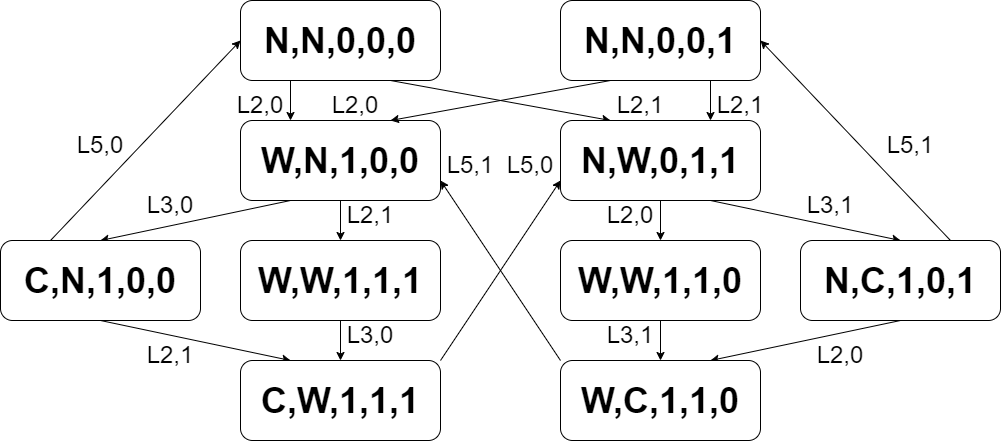
\includegraphics[width=0.8\textwidth]{image/hw1-3-1.drawio.png}
    \caption{State Transition Graph for Part 1}
    \label{fig:hw1-3-1}
\end{figure}

\subsection{Part 2}

As you can see in the image, there is not a state where $C_0$ and $C_1$ happen at the same time.

\section{Problem 4}

\subsection{Part 1}

Example of a iteration:

\begin{enumerate}
    \item Before start of the iteration:
        $y_1 = 0$ and $y_2 = x$.
        $P_1$ is about to execute $y_1 = y_2 + 1$.
        $P_2$ is about to execute $y_2 = 0$.
    \item $P_1$ executes $y_1 = y_2 + 1$.
        Now $y_1 = x + 1, y_2 = x$.
    \item $P_2$ executes $y_2 = 0$ (finishes the critical section).
        Now $y_1 = x + 1, y_2 = 0$.
    \item $P_2$ executes $y_2 = y_1 + 1$.
        Now $y_1 = x + 1, y_2 = x + 2$.
    \item $P_1$ tests $y_2 = 0 \vee y_1 < y_2$.
        It is true, so $P_1$ enters the critical section.
    \item $P_1$ finishes the critical section, and set $y_1 = 0$.
        Now $y_1 = 0, y_2 = x + 2$.
    \item $P_2$ tests $y_1 = 0 \vee y_2 < y_1$.
        It is true, so $P_2$ enters the critical section.
    \item Now, $P_1$ is about to execute $y_1 = y_2 + 1$,
        and $P_2$ is about to execute $y_2 = 0$, the start of another iteration.
\end{enumerate}

As long as we can reach the start of some iteration, we can get into an infinite loop.
During each iteration, the value of $y_2$ will grow by $2$, which indicates an infinite transition system,
since the state of the system is unbounded.

So, we just need to prove that we can arrive at the start of some iteration.

Consider the following steps:

\begin{enumerate}
    \item At first, $y_1 = y_2 = 0$.
    \item $P_2$ executes $y_2 = y_1 + 1$.
        Now $y_1 = 0, y_2 = 1$.
    \item $P_2$ tests $y_1 = 0 \vee y_2 < y_1$.
        It is true, so $P_2$ enters the critical section.
    \item Now, it is the start of an iteration where $x = 1$.
\end{enumerate}

In conlusion, the value of $y_2$ can grow arbitrarily large, resulting in an infinite transition system.

\subsection{Part 2}

Proof by contradiction. If both $P_1$ and $P_2$ enters the critical section, then we have:

$$
(y_2 = 0 \vee y_1 < y_2) \wedge (y_1 = 0 \vee y_2 < y_1)
$$

Since at most one in $y_1 < y_2$ and $y_2 < y_1$ can be true, we have at least $y_1 = 0$ or $y_2 = 0$.
Due to the symmetry of the two programs, without loss of generality, we assume $y_2 = 0$.

First of all, it's trivial to see $y_1 \ge 0$ and $y_2 \ge 0$, which can be proved by induction
(each write to $y_1$ or $y_2$ is non-negative, whatever the sequence of the writes is).

In addition, the last write to $y_2$ before $P_2$ enters the critical section is $y_2 = y_1 + 1$,
so we have $y_2 \ge 0 + 1 = 1$, which contradicts the assumption $y_2 = 0$.

As a result, we have proved that $P_1$ and $P_2$ cannot enter the critical section at the same time.

\chapter{Homework 2}

\section{Problem 1}

There are 2 kinds of traces:

\begin{itemize}
    \item \textbf{Trace 1:} $\{a\}, \{a\}, \{a, b\}, \{a\}, \{a, b\}, \{a\}, \cdots$
    \item \textbf{Trace 2:} $\{a\}, \emptyset, \{a, b\}, \{a\}, \{a, b\}, \{a\}, \cdots$
\end{itemize}

Type 1 starts with 2 $\{a\}$, and then alternates between $\{a, b\}$ and $\{a\}$.
Type 2 starts with $\{a\}$ and $\emptyset$, and then alternates between $\{a, b\}$ and $\{a\}$.

\section{Problem 2}

To show that a property is a safety property, we need to show each trace that violates the property has a bad prefix.

Otherwise, the property is not a safety property.

Specially, we may use the fact that an invariant is a safety property.

\subsection{a}

\newcommand{\A}{\{A\}}
\newcommand{\B}{\{B\}}

$$
P = \{A_0 A_1 A_2 \cdots A_n \cdots | \forall i \ge 0,  A \notin A_n \}
$$

It's trivial that $P$ is a safety property (it is even an invariant, where $\Phi = \{\B, \emptyset \}$).

\subsection{b}

Consider the following trace:

$$
T = \{\B \B \B \cdots \}
$$

It is composed of infinitely many $\B$. Obviously, it is not satisfied by the given property.
Moreover, for every finite prefix $T_n = \{\B \B \B \cdots \B\}$ with $n$ $\B$,
there exists a trace $\{\B \B \B \cdots \B \A \B \B \cdots\}$
that starts with $T_n$ and satisfies the property $P$.

As a result, the property is not a safety property, as $T$ does not have a bad prefix.

\subsection{c}

$$
P = \{ (\A \B)^\omega, (\B \A)^\omega \}
$$

Trivially, for any trace that violates the property, there exists a bad prefix $T$
which ends with $\A \A$ or $\B \B$ or $\{A, B\}$ or $\emptyset$.
(Otherwise, in this trace each $\A$ must be followed by $\B$, and vice versa, which must be in $P$.)

In short, the property is a safety property.

\subsection{d}

Similar to (b), consider the following trace:

$$
T = \{\A \A \A \cdots \}
$$

Similar to (b), we can prove that it has no bad prefix.

As a result, the property is not a safety property.

(In fact, it is a liveness property, though I don't want to prove it here.
Since the only property which is both a safety property and a liveness property is $(2^{AP})^\omega$,
and this property is of course not $(2^{AP})^\omega$, so we may conclude that it is not a safety property
in an alternative way.)

\section{Problem 3 (wrong version)}

\newcommand{\pref}{\textit{prefix}}

Review the definition of liveness property:
An LT property $P \subseteq (2^{AP})^\omega$ is a liveness property if we have that
$\pref(P) = (2^{AP})^*$, where $\pref(-)$ is the set of finite prefixes in $P$.

\subsection{a}

If $P, P'$ are both liveness property, then $P \cup P'$ is also a liveness property.
This is because:

$$
\begin{aligned}
    \pref(P \cup P')
    &= \{ A_0 A_1 \cdots A_n | A_0 A_1 \cdots A_n \cdots \in P \cup P' \} \\
    &\supseteq \{ A_0 A_1 \cdots A_n | A_0 A_1 \cdots A_n \cdots \in P \} \\
    &= \pref(P) \\
    &= (2^{AP})^* \\
\end{aligned}
$$

In addition, we have $\pref(P \cup P') \subseteq (2^{AP})^*$, so $\pref(P \cup P') = (2^{AP})^*$,
which indicates that $P \cup P'$ is a liveness property.

\subsection{b}

If $P, P'$ are both liveness property, then $P \cap P'$ may not be a liveness property.
Consider the following counterexample:

$AP = \A$. For simplicity, we denote $\A$ as $1$ and $\emptyset$ as $0$. We construct $P, P'$ as follows:

$$
P  = \{ (0 | 1)^n 1 1 1 \cdots \}
P' = \{ (0 | 1)^n 0 0 0 \cdots \}
$$

Intuitively, $P$ requires that each trace ends with infinitely many $1$,
while $P'$ requires that each trace ends with infinitely many $0$.

It's easy to see that $P \cap P' = \emptyset$, which is not a liveness property
(since its prefix set is $\emptyset$).

\section{Problem 3}

Sorry, I was wrong. I need to prove about safety properties, not liveness properties.

\subsection{a}

If $P, P'$ are both safety property, then $P \cup P'$ is also a safety property.
This is because:

\newcommand{\bad}[1]{\textit{BadPrefix}(#1)}
\newcommand{\whole}{(2^{AP})^\omega}

For every word $\sigma \in \whole \setminus (P \cup P')$,
since $\whole \setminus (P \cup P') \subseteq \whole \setminus P$
and $\whole \setminus (P \cup P') \subseteq \whole \setminus P'$,
we have prefixes $\hat{\sigma_1}$ and $\hat{\sigma_2}$ such that
$\hat{\sigma_1} \in \bad{P}$ and $\hat{\sigma_2} \in \bad{P'}$.

Now, it is easy to see that the longer one in $\hat{\sigma_1}$ and
$\hat{\sigma_2}$ is also a bad prefix of $P \cup P'$.

This proves that $P \cup P'$ is a safety property,
since every trace outside $P \cup P'$ has a bad prefix.

\subsection{b}

If $P, P'$ are both safety property, then $P \cap P'$ is also a safety property.
This is because:

$$
\sigma \in \whole \setminus (P \cap P')
= (\whole \setminus P) \cup (\whole \setminus P')
$$

As a result, for each $\sigma \in \whole \setminus (P \cap P')$,
without loss of generality, we may assume $\sigma \in \whole \setminus P$,
which indicates that there exists a bad prefix $\hat{\sigma} \in \bad{P}$.

Now it is easy to see that $\hat{\sigma}$ is also a bad prefix of $P \cap P'$.

This proves that $P \cap P'$ is a safety property,
since every trace outside $P \cap P'$ has a bad prefix.

\section{Problem 4}

\subsection{a}

\newcommand{\aaa}{\{\alpha\}}
\newcommand{\bb}{\{\beta\}}
\newcommand{\ee}{\{\eta\}}
\newcommand{\Act}{\textit{Act}}

First of all, since it is unconditionally $\aaa$-fair, we must visit $\aaa$ infinitely many times.
As a result, we cannot reach $s_4$, as it will result in an infinite loop which only takes action
$\bb$, which violates the fairness condition.

Moreover, since it is strongly $\ee$-fair, we can only visit $s_3$ finitely many times.
If we visit $s_3$ infinitely many times, then according to the fairness condition,
since $\ee \subseteq \Act(s_3)$, there must be infinitely many $\ee$ actions taken.
However, once $\ee$ is taken, we will reach $s_4$, which is against the previous conclusion.

Therefore, for each fair path $T=\{s_0 s_1 s_2 \cdots\}$, there exists some $m$, such that
$\forall n \ge m, s_n \ne s_3$.

Next, we claim that a fair path must visit $s_0$ infinitely many times.
If not, then there exists some $q$ such that $\forall n \ge q, s_n \ne s_0$.
Consider the states after $\max(m, q)$, it is clear that we can only end up
visiting $s_1$ continuously. This violates the strongly $\{delta, \gamma\}$-fair condition,
since $\{delta, \gamma\} \cup \Act(s_1) = \{\gamma\} \ne \emptyset$, which means
that we must take infinitely many $\delta$ or $\gamma$, which is contradictory to the fact
that we end up visiting $s_1$ continuously.

As a result, a fair path must visit $s_0$ infinitely many times. We may apply the strongly $\bb$-fair condition,
which shows that we must take action $\bb$ infinitely many times, equivalently visiting $s_2$ infinitely many times.

Then, we claim that:

$$
\textit{TS} \models_{\mathcal{F}_1} P_2
$$

This is because for each fair path, it will visit $s_2$ infinitely many times,
which means $\{a, b\}$ will appear infinitely many times in a fair trace.

In addition, after $m$ steps, we can only reach $s_0, s_1, s_2$.
Then if $a \in {A_k}, k \ge m$, then we must be in $s_0$ or $s_2$.
Whichever state we are in, we will take action and transfer to $s_1$ or $s_2$,
where $\{b\}$ will be in $A_{k+1}$.

As a result, we have shown that each fair trace is in $P_2$, which means
$\textit{TS} \models_{\mathcal{F}_1} P_2$

\subsection{b}

Consider the following counterexample:

\newcommand{\xa}{\xrightarrow{\alpha}}
\newcommand{\xb}{\xrightarrow{\beta}}
\newcommand{\xg}{\xrightarrow{\gamma}}
\newcommand{\xd}{\xrightarrow{\delta}}

$$
T = \{s_0 \xb s_2 \xd s_3 \xa s_1 \xg s_0 \xb s_2 \xd s_3 \xa s_1 \xg \cdots\}
$$

It's easy to verify that the trace of $T$ is $\mathcal{F}_2$ fair, and it is not in $P_2$.

Therefore, $\textit{TS} \not\models_{\mathcal{F}_2} P_2$

\chapter{Homework 3}

\section{Problem 1}

\subsection{a}

\begin{figure}[H]
    \centering
    \includegraphics[width=0.8\textwidth]{generated/hw3/p1_a_0.pdf}
\end{figure}

\begin{figure}[H]
    \centering
    \includegraphics[width=0.8\textwidth]{generated/hw3/p1_a_1.pdf}
\end{figure}

\subsection{b}

\begin{figure}[H]
    \centering
    \includegraphics[width=0.8\textwidth]{generated/hw3/p1_b_0.pdf}
\end{figure}

\begin{figure}[H]
    \centering
    \includegraphics[width=0.8\textwidth]{generated/hw3/p1_b_1.pdf}
\end{figure}

\section{Problem 2}

\subsection{c}

\begin{figure}[H]
    \centering
    \includegraphics[width=0.8\textwidth]{generated/hw3/p2_c.pdf}
\end{figure}

\subsection{l}

\begin{figure}[H]
    \centering
    \includegraphics[width=0.8\textwidth]{generated/hw3/p2_l.pdf}
\end{figure}

\section{Problem 3}

\begin{figure}[H]
    \centering
    \includegraphics[width=0.8\textwidth]{generated/hw3/p3.pdf}
\end{figure}

\section{Problem 4}

\subsection{a}

\begin{figure}[H]
    \centering
    \includegraphics[width=0.8\textwidth]{generated/hw3/p4_a.pdf}
\end{figure}

\subsection{b}

Remark: this is converted automatically by an algorithm implemented in python.

\begin{figure}[H]
    \centering
    \includegraphics[width=0.8\textwidth]{generated/hw3/p4_b.pdf}
\end{figure}

\chapter{Homework 4}

\section{Problem 1}

\begin{figure}[H]
    \centering
    \includegraphics[width=0.8\textwidth]{generated/hw4/p1.pdf}
\end{figure}

\section{Problem 2}

\subsection{a}

The $\omega$-regular expression is:

$$
(A (A + B + C)^* A + C (A + B + C)^* C)^{\omega}
$$

\subsection{b}

The $\omega$-regular expression is:

$$
(B + C)^*((B + A(BC)^*B)A^{\omega} + A(BC)^{\omega})
$$

\section{Problem 3}

\begin{figure}[H]
    \centering
    \includegraphics[width=0.8\textwidth]{generated/hw4/p3.pdf}
\end{figure}

\chapter{Homework 5}

\section{Problem 1}

\begin{enumerate}
    \item (a) $\bigcirc$ a: $\{s_1, s_2, s_3, s_4\}$
    \item (b) $\bigcirc \bigcirc \bigcirc$ a: $\{s_1, s_2, s_3, s_4\}$
    \item (c) $\square$ b: $\emptyset$
    \item (d) $\square$ $\Diamond$ a: $\{s_1, s_2, s_3, s_4\}$
    \item (e) $\square$ (b $\cup$  a): $\emptyset$
    \item (f) $\Diamond$ (a $\cup$ b): $\{s_1, s_2, s_3, s_4\}$
\end{enumerate}

\section{Problem 2}

\newcommand{\TS}{\text{TS}}

\begin{enumerate}
    \item $\TS \not \models \varphi_1 = \Diamond$ $\square$ $c$
    \item $\TS \models \varphi_2 = \square$ $\Diamond$ $c$
    \item $\TS \models \varphi_3 = \bigcirc$ $\neg c$ $\rightarrow \bigcirc$ $ \bigcirc$ $c$
    \item $\TS \not \models \varphi_4 = \square$ $a$
    \item $\TS \models \varphi_5 = a$ $\bigcup$ $\square$ $(b \vee c)$
    \item $\TS \not \models \varphi_6 = (\bigcirc \bigcirc b)$ $\bigcup$ $(b \vee c)$
\end{enumerate}

counterexample for $\varphi_1$: $\pi = s_1 s_3 s_4 s_3 s_4 s_3 \cdots$  (infinite $s_4$ and $s_3$ loop)

for $\varphi_2$: all cycles in the graph contains $c$

for $\varphi_3$: if next state does not satisfy $c$, then the next state must be $s4$,
and we have $\text{Post}(s_4) \models c$

counterexample for $\varphi_4$: $\pi = s_2 \cdots$ (can be any path starting from $s_2$)

for $\varphi_5$: only $s_1$ does not satisfy $(b \vee c)$ and $s_1 \models a$, and we can only reach
$s_1$ at the beginning.

counterexample for $\varphi_6$: $\pi = s_1 s_4 s_2 \cdots$ (can be any path with such a prefix)


\printbibliography[heading=bibintoc, title=\ebibname]
\appendix

\end{document}
